\scanpage{106}
% Archive pencil foliation: 105.%
i.e. que la filtration dudit foncteur a\unsure{\deleted{m}d|\deleted{d}m|d}\unsure{\deleted{d}m|\deleted{m}d}et un\deleted{e} splittage compatible avec les produits tensoriels. Mais le choix d'un tel spl\unsure{\deleted{n}i|\deleted{i}n|\rlap{i}i}ttage équivaut à celui d'un point \deleted{sous} sur un certain torseur à droite $Q=Q'$ sous le \inserted{\rlap{\handwritten{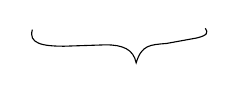
\begin{tikzpicture}[baseline=-.2ex,x=1em,y=1em]
\draw (-.15,.6) .. controls (-.3,.1) and (.2,0) .. (1,0) -- (2.5,.05) .. controls (3.1,.05) and (3.5,-.1) .. (3.6,-.6) .. controls (3.8,.05) and (4.1,.05) .. (4.7,.1) -- (5.8,.3) .. controls (6.2,.4) and (6.2,.5) .. (6.1,.65);
\end{tikzpicture}}}schéma en} groupe\unsure{s} \inserted{\rlap{\handwritten{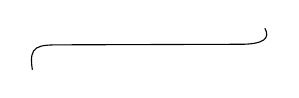
\begin{tikzpicture}[baseline=-.2ex,x=1em,y=1em]
\draw (-.4,-.8) .. controls (-.55,.1) and (-.2,.1) .. (.7,.1) -- (7,.12) .. controls (8,.1) and (8.2,.35) .. (8,.7);
\end{tikzpicture}}}(pro-unipotent)} $H$ des automorphismes de $F$ respectant la filtration et induisant l'identité sur le gradué associé; il n'est pas du tout canonique !

3) Appelons \uline{pré-str\unsure{\deleted{cu}uc|\deleted{uc}cu|ac}ture de Hodge} sur un espace vectoriel \inserted{\rlap{\handwritten{\begin{tikzpicture}[baseline=-.2ex,x=1em,y=1em]
\draw (.1,-.65) .. controls (0,-.35) and (.6,.05) .. (1.2,.7) -- (1.6,1.3);
\end{tikzpicture}}}$V$} de dimension finie sur $\underline{Q}$, la donnée d'une bigraduation sur $V\otimes_{\underline{Q}}\underline{C}=V_{\underline{C}}$, $V_{\underline{C}}=\handwritten{\coprod_{p,q}}V^{p,q}$, telle que a) la graduation totale correspondante soit ``définie sur $\underline{Q}$'' \uline{i.e.} $\handwritten{\coprod}_{p+q=n}V^{p,q}$ provienne d'un sous espace $V_{\underline{Q}}^n$ de $V$, et b) on a $\overset{\handwritten{\rule{.65em}{.35pt}}}{V}^{p,q}=V^{q,p}$, où \begin{tikzcd}[cramped]x\arrow[r,mapsto]&\overset{\handwritten{\rule{.55em}{.35pt}}}{x}\end{tikzcd} désigne la conjuguaison complexe. \unsure{\deleted{\unsure{p|ç}}(|\deleted{(}\unsure{p|ç}}NB Généralisation à des corps plus généraux laissée à Saavedra). Les vectoriels $V$ munis d'une pré-structure de Hodge forment une catégorie tensorielle sur $\underline{Q}$ dans un sens évident, muni d'un foncteur fibre canonique, le foncteur ``oubli''\inserted{\rlap{\handwritten{\begin{tikzpicture}[baseline=-.2ex,x=1em,y=1em]
\draw (.7,.5) .. controls (1.05,-.2) and (.2,-.35) .. (-.4,-.9);
\end{tikzpicture}}}$F$}. On trouve donc un groupe de \unsure{\rlap{G}G|\deleted{g}G|\deleted{G}g}alois $G$, et \deleted{tout} plus généralement toute \inserted{\rlap{\handwritten{\begin{tikzpicture}[baseline=-.2ex,x=1em,y=1em]
\draw (-.25,-.7) .. controls (0,-.25) and (.6,-.15) .. (1.25,-.1) .. controls (1.65,0) and (1.6,.35) .. (1.5,.6);
\end{tikzpicture}}}$\otimes$-}sous-catégorie $\underline{C}$ de la catégorie précédente nous définit un groupe de Galois $G$. La bigraduation sur le foncteur \deleted{oubli} $F_{\underline{C}}(V)=V\otimes_{\underline{Q}}\underline{C}$ correspond, en vertu de 1) (où il convient cependant de se permettre une extension du corps de \unsure{\deleted{h}b|\deleted{b}h|\rlap{b}b}ase sur le foncteur fibre envisagé ....) d'un homomorphisme \begin{tikzcd}[cramped]{\underline{G}_m}_{\underline{C}}^2\arrow[r]&G_{\underline{C}}\end{tikzcd}, i.e. de deux homomorphismes \inserted{\rlap{\handwritten{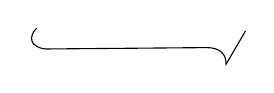
\begin{tikzpicture}[baseline=-.2ex,x=1em,y=1em]
\draw (-.15,.65) .. controls (-.45,.35) and (-.4,-.05) .. (.2,-.1) -- (6,-.05) .. controls (6.5,-.05) and (6.7,-.3) .. (6.7,-.65) -- (7.4,.55);
\end{tikzpicture}}}qui commutent}
\diagram{$i_1,i_2:$\begin{tikzcd}[cramped]{\underline{G}_m}_{\underline{C}}\arrow[r]&G_{\underline{C}}.\end{tikzcd}}
Les deux conditions a) et b) imposées aux structures envisagées s'interprètent respectivement par les faits que l'homomorphisme
\diagram{\begin{tikzcd}[cramped]i_{\underline{C}}=i_1i_2\unsure{\doteqdot|\deleted{:}=|\deleted{;}=|\deleted{=}:|\deleted{=};}\handwritten{\lambda}\arrow[r,mapsto]&i_1\handwritten{(\lambda)}i_2\handwritten{(\lambda)}\end{tikzcd}}
est ``défini sur $\underline{Q}$'' i.e. provient d'un homomorphisme
\diagram{$i:$\begin{tikzcd}[cramped]\underline{G}_m\arrow[r]&G,\end{tikzcd}}
\margin{\tikz[baseline=0pt,x=1em,y=1em]{\draw (0,0) .. controls (.1,.05) and (.17,.15) .. (.22,.3);}}(nécessairement central, car les composantes homogènes $V_{\underline{Q}}^n$ d'une pré-structure de Hodge sont \deleted{nécessairement}\inserted{évidemment} munis d'une \inserted{\rlap{\handwritten{\begin{tikzpicture}[baseline=-.2ex,x=1em,y=1em]
\draw (.6,-.55) .. controls (.8,-.25) and (1.1,-.15) .. (1.4,-.05);
\end{tikzpicture}}}pré-}structure de Hodge de façon que $V$ so\rlap{i}it la somme directe de $V_{\underline{Q}}^n$ en tant que pré-structure

